\chapter{Bringing Storm to Multi-core}

The following chapter explains the design of Storm-MC. We describe how Apache Storm behaves on multi-core machines (\ref{sec:storm_on_mc}), how the Storm architecture was ported over to multi-core (\ref{sec:storm_mc_arch}), how tuple processing was ported to multi-core (\ref{sec:tuple_processing}), and finally, we list feature differences between Apache Storm and Storm-MC (\ref{sec:differences}).

The design of Storm-MC was ported over from Apache Storm. This enabled rapid progress while guaranteeing compatibility with the Apache Storm API. Clearly, however, some differences had to be made to take advantage of multi-core machine performance implications. 

\section{Apache Storm on Multi-core}
\label{sec:storm_on_mc}

To begin, we discuss why Apache Storm does not perform optimally on a single multi-core machine. Storm can be ran in local mode where it emulates execution on a cluster. This mode exists so that it is possible to debug and develop topologies without needing access to a cluster. However, there are several reasons why the local mode is not as performant as it could be.

\subsection{Tuple processing}

Figure \ref{fig:worker_inside} shows how tuple processing is implemented inside a Storm worker process. The tuple is read from a message buffer by the receiver thread of the worker and put on a receive queue of the corresponding executor. The tuple is then picked up by the component thread of the executor for task execution.

After the component thread has executed the task it puts the tuple on the executor sender queue. There, it is picked up by the executor sender thread which puts the tuple on the global sender queue of the worker. Lastly, the global sender thread of the worker serialises the tuple and sends it downstream.

Alternatively, if the tuple is forwarded to an executor in the same worker process it is put on the receiver queue of the corresponding executor directly after processing.

\begin{figure}[!htb]
	\centering
	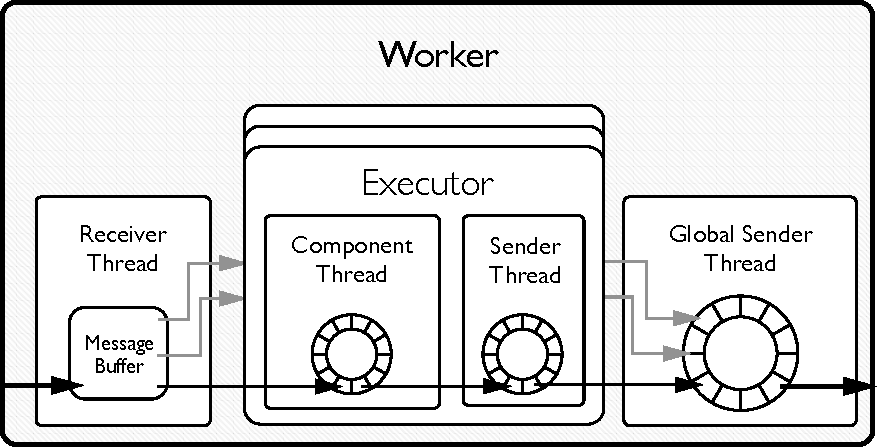
\includegraphics[scale=0.7]{pdf/worker_inside.pdf}
	\caption{Tuple processing in Apache Storm.}
	\label{fig:worker_inside}
\end{figure}

Storm uses the term "queue" freely but in fact the queues are implemented as ring buffers using the LMAX Disruptor library \cite{LMAXDisruptor}. Detailed background on how Disruptor works and its performance benchmarks can be found in \cite{Thompson_Farley_Barker_Gee_Stewart_2011}.

There is a lot of overhead necessary to simulate sending tuples to executors in other worker nodes. For one, there is significant overhead from the tuple passing through the three queues of a worker. In \cite{DisruptorWiki}, the authors of LMAX Disruptor show that a three step pipeline has half the throughput of a single consumer-producer pipeline.

Furthermore, Storm simulates the cluster network by running a local Netty \cite{Netty} server.

\subsection{Heartbeats \& Timers}

Additionally, every worker has a heartbeat thread that simulates sending heartbeat messages to the Nimbus process. It does this by writing to a local cache which is persisted to a file by a blocking write on every heartbeat. While heartbeats are essential in cluster mode, there is no need for them in local mode.

\subsection{Acker \& System Bolts}

The acker and system bolts are ran for every topology. The acker bolt can be disabled via the configuration file. In such a case it executes idly.

\subsection{Zookeeper}

Another overhead is running a local Zookeper server which emulates the Zookeeper nodes of a cluster. Running the Zookeeper server is a massive addition to the list of overheads. Indeed, during profiling we found that a topology with one worker and three executors was being executed with 55 threads (not including system JVM threads and threads created by the profiler). 28 of these threads were started by Zookeeper. Table \ref{table:breakdown} shows what the individual threads were used for.

\begin{table}[h!]
\centering
\begin{tabular}{@{}lc@{}}
    \textbf{Spout Parallelism} & \textbf{\# of Threads} \\ \toprule
    Main Thread & 1  \\
	Worker Sender \& Receiver Threads & 2  \\
    Acker \& System Component Threads & 2  \\
    Executor Component Threads & 3  \\
    Executor Sender Threads & 5  \\
    Various Timers \& Event Loops & 13  \\
    Zookeper Server & 28  \\
\end{tabular}
\caption{Break-down of threads used by Apache Storm to execute a topology with 3 components.}
\label{table:breakdown}
\end{table}

To find out what state the threads were actually in at any given time we run the topology and recorded a thread dump every second for five minutes. The results can be observed in table \ref{table:dump}.

\begin{table}[h!]
\centering
\begin{tabular}{@{}lc@{}}
    \textbf{Spout Parallelism} & \textbf{\# of Threads} \\ \toprule
    RUNNABLE & 8  \\
	TIMED WAITING & 22  \\
    WAITING & 25  \\
\end{tabular}
\caption{Recorded thread states over five minute period.}
\label{table:dump}
\end{table}

<<dump-plot, echo=FALSE, cache=TRUE, fig.cap="Threads over time.", fig.align="center", fig.height=3>>=
@

As can be seen from the table, most of the threads were either in state \texttt{WAITING} or \texttt{TIMED WAITING}. According to the Java documentation on thread states \cite{JavaThreads} these two states are used for threads that are waiting for an action from a different thread and cannot be scheduled by the scheduler until that action is executed.

In the subsequent sections we will discuss how the number of running threads was significantly reduced. In fact, to execute the same topology on Storm-MC would only require 5 threads.

\todo{Plot threads vs components}
\todo{Maybe include Thread Dump and a graph of thread counts}

%	\item[Fault Tolerance] \hfill \\
%	Storm is made to be fault-tolerant. This means that it can guarantee a tuple being processed from its spout all the way to its final bolt. To do this it adds an additional acker bolt to every topology. This bolt acts as a root of a tree with the nodes being all the components the tuple "goes" through. If the tuple gets successfully processed by a component its node is marked as "acked". Hence once all nodes of the tree are marked as "acked" Storm can guarantee the tuple was processed.
%	\item[Redundant threads] \hfill \\
%	Storm runs many threads which are only useful in distributed context. Indeed, during our experiments we found that a topology with 8 executors was being executed with 64 threads. This included threads which were used as timeout timers or to send heartbeats and were unnecessary in a multi-core setting. Obviously, not all of them were executing in parallel but there is clearly room for reduction.

\section{Storm-MC Architecture}
\label{sec:storm_mc_arch}

\todo{Probably don't call this Architecture}

The design we adopted for porting worker nodes is to only have one worker process running all the executor threads of a topology.

Additionally, the code for the Nimbus daemon was merged with the worker. This was done because there is no need to run the Nimbus and worker specific code at the same time. Once Nimbus sets up the topology, all the work is done by the worker. Hence they can be executed serially.

\subsection{Nimbus}

Unlike Nimbus executing on a Storm cluster, Nimbus in Storm-MC does not support running multiple topologies at the same time. However, to do that one only needs to run the topology in a separate process. This is because unlike when executing on the cluster different topologies do not need to share any state and it is more natural to execute them as separate processes.

This has the added benefit of each process having its own part of main memory thus reducing cache conflicts as shown in \cite{Chandra:2005:PIC:1042442.1043432} and providing higher security by not having different topologies share memory space. Additionally, if a single thread of one topology is blocking it does not block other topologies.

Nimbus on Storm-MC does not support scheduling topologies. Since within one process there is only one topology running at a time and the hardware configuration of the machine does not change, the parallelism is clearly defined by the number of executors per component specified in the topology configuration.

One way to implement scheduling could be to pin threads to specific cores. Unfortunately, Java does not provide support for CPU affinity, the assignments are handled automatically by the JVM. Potentially, this could be achieved by using C or C++, both of which support CPPU affinity, but this was not implemented in Storm-MC.

\todo{Mention porting over from Thrift.}

The role of Nimbus in Storm-MC has effectively been reduced to validating the topology and passing it along to the worker part of the process which handles the topology execution.

\subsection{Worker}

In Apache Storm, a worker node runs the supervisor daemon, which in turns launches worker processes which contain executor threads which contain tasks. In Storm-MC, however, there is only one worker process which contains all the executor threads and their tasks.

This design has several benefits:

\begin{itemize}
	\item All the inter-thread communication is occurring within one Worker.
	\item Supervisor can be removed as there is no need to synchronise workers.
	\item There is no need to simulate over-the-network message passing.
	\item Message passing between executor threads within a worker stays the same as in Apache Storm.
\end{itemize}

A comparison of an Apache Storm worker node and its Storm-MC equivalent can be seen in figure \ref{fig:comparison}.

\begin{figure}[!htb]
\centering
\begin{subfigure}{.5\textwidth}
  \centering
  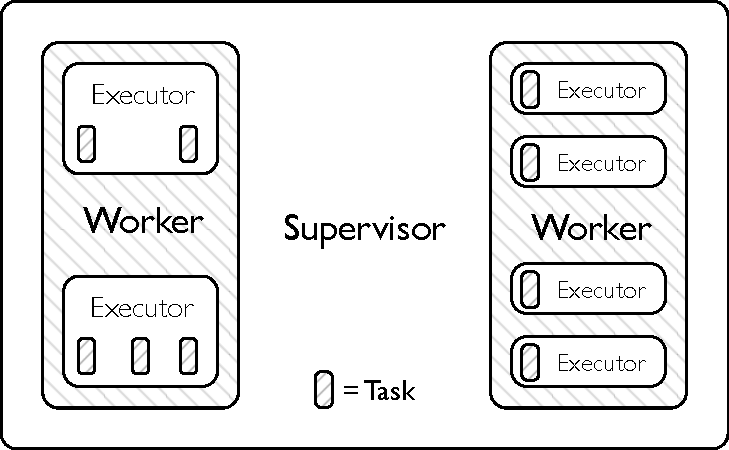
\includegraphics[width=0.95\linewidth]{pdf/distributed_worker.pdf}
  \caption{Worker in Apache Storm.}
  \label{fig:comparison1}
\end{subfigure}%
\begin{subfigure}{.5\textwidth}
  \centering
  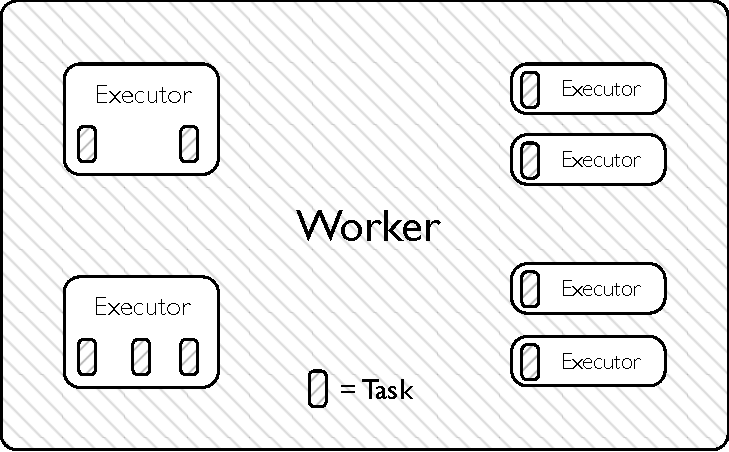
\includegraphics[width=0.95\linewidth]{pdf/local_worker.pdf}
  \caption{Worker in Storm-MC.}
  \label{fig:comparison2}
\end{subfigure}
\caption{Comparison of a worker in Storm and Storm-MC}
\label{fig:comparison}
\end{figure}

\subsection{State}

In light of previous subsections Storm-MC is completely stateless. The cluster state that was managed by Zookeeper in Apache Storm was completely stripped away. This state was only relevant when multiple topologies were sharing the cluster.

\section{Tuple Processing}
\label{sec:tuple_processing}

\todo{Mention overhead by running SystemBolt vs just timer in Storm-MC}

\begin{figure}[!htb]
	\centering
	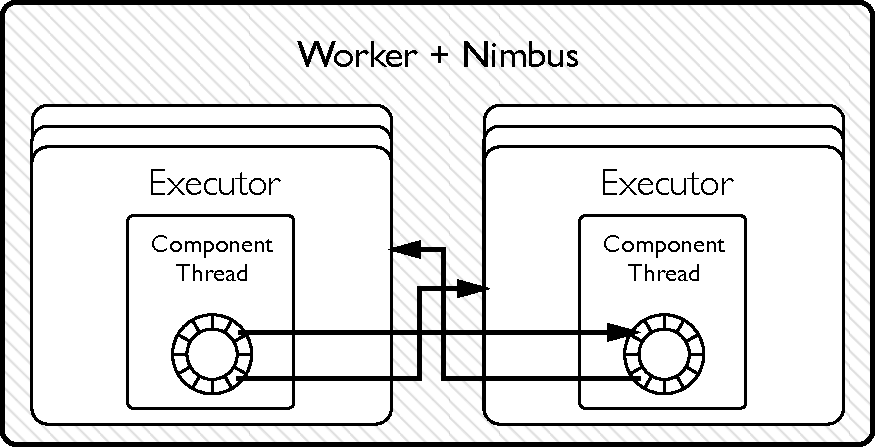
\includegraphics[scale=0.7]{pdf/worker_inside_mc.pdf}
	\caption{Tuple processing in Storm-MC.}
	\label{fig:worker_inside_mc}
\end{figure}

The implementation of tuple processing in Storm-MC can be seen in figure \ref{fig:worker_inside_mc}. As can be seen from the figure, the queues used for remote message sending were stripped away and there is only one Disruptor queue for every executor. Once an executor is done processing a tuple it simply puts it on the Disruptor queue of the bolts downstream.

There were several other options we considered when implementing tuple processing. However, the Disruptor shows superior throughput and latency compared to alternative solutions in \cite{something}.

\todo{find the citation for above claim.}

\section{Differences between Apache Storm and Storm-MC}
\label{sec:differences}

\todo{Maybe present this as a table of features.}
